 \documentclass{article}
\usepackage{amsmath}
\usepackage{amsthm}
\usepackage{amssymb}
\usepackage{graphicx}
\usepackage{float}
\usepackage[dutch]{babel}
\usepackage[margin=3.5cm]{geometry}
\usepackage{etoolbox}
\usepackage{textcomp}
\usepackage{gensymb}
\usepackage{changepage}
\usepackage{enumitem}
\usepackage{fancyhdr}
\usepackage{url}
\usepackage{apacite}
\usepackage{verbatim}
\usepackage{bm}
\usepackage{eurosym}
\usepackage{minted}
\usepackage{color}
\usepackage{listings}
\usepackage{subfig}
\usepackage[font=footnotesize,labelfont=bf]{caption}
\usepackage[utf8]{inputenc}
\usepackage{titlesec}
\usepackage{sectsty}
\usepackage{lipsum}
\usepackage{hyperref}
\usepackage{epigraph}
\usepackage{wrapfig}
\usepackage[nottoc]{tocbibind}
\usepackage{biblatex}
\addbibresource{bibliography.bib}

%hyperrefs
\hypersetup{
    colorlinks=true,
    linkcolor=blue,
    filecolor=magenta,      
    urlcolor=cyan,
}
\urlstyle{same}

%commands
\newcommand*\dif{\mathop{}\!\textnormal{\slshape d}}
\newcommand{\dd}[2]{\frac{\partial #1}{\partial #2}}
\newcommand{\ddn}[3]{\frac{\partial^{#3}#1}{{\partial #2}^{#3}}}
\newcommand{\note}[1]{\textbf{\color{red}{#1}}}
%1D assumption
\newcommand{\myeq}[1]{\mathrel{\stackrel{\makebox[0pt]{\mbox{\normalfont\tiny #1}}}{=}}}
\newcommand{\overEquals}[1]{\myeq{#1}}
%vectors thick instead of arrow
\renewcommand{\vec}[1]{\mathbf{#1}}
\newcommand{\limx}{\lim_{\Delta x \to 0}}

\begin{document}
	\title{[Algen]}
	\author{Joost Bus\\
	        Rona Roovers\\
	        Joost Imhof\\
			Billy Verhage
			}
	\date{}
	\maketitle
	\vfill
	\noindent
	TU Delft \hfill \today \\
	Faculteit EWI\\ \hfill Delft
	BSc Technische Wiskunde \hfill Supervisor: Prof. dr. ir. A.W. Heemink 
	
	\fancyhf{}
	\fancyhead[C]{\thepage}
	\pagestyle{fancy}
	\renewcommand{\headrulewidth}{0pt}
	\newcommand{\odds}{\textnormal{odds}}

	\pagenumbering{roman}
	\thispagestyle{empty}
	
	\newpage
	
	\newpage
	\setcounter{tocdepth}{2}
	\tableofcontents
	\section*{Abstract}
\addcontentsline{toc}{section}{Abstract}

Hallo
	
	\newpage
	\pagenumbering{arabic}
	\setcounter{page}{1}
	\section{Introductie}
Elke na zomer slippen de grachten van Delft dicht met kroos. Kroos is een familie van planten die zich niet wortelen in de bodem. Kroos drijft met blaadjes, de grootte varieert erg per soort, op het wateroppervlak. Kroos kan goed bloeien in stil staand water. Algen kunnen juist beter bloeien in stromend water. Waaronder grote open water lichamen zoals de Noordzee of oceanen. Hier hebben algen een moordende invloed. Een plaag van algen of kroos kan veroorzaakt worden door een overschot aan nutriënten, wat kan ontstaan door bijvoorbeeld overbemesting. Bij een overschot aan nutriënten zoals stikstof en fosfaten is er geen concurrentie meer over deze stoffen. Hierdoor kunnen algen exponentieel groeien. Een dichte algen[Hey Hey HEY wil je even naar de chat kijken? Groetje Billy vanuit het vliegtuig] -laag kan zorgen voor het tegenhouden van licht en zuurstof. Door het gebrek aan licht zullen andere planten afsterven, waardoor het zuurstof gehalte van het water nog verder afneemt. Zonder zuurstof in het water zullen vissen en andere organismen niet meer kunnen overleven. Het eco-systeem zal bijna helemaal uitsterven. Dit proces heet eutrofiëring. Net zoals in Figuur \ref{fig:bloom} zijn er over de hele wereld lichamen van water die uitsterven. De bacteriën die algen verteren verbruiken in het geval van een plaag alle zuurstof in het water. Deze bacteriën kunnen ook enorm toe nemen in populatie omdat er zo veel algen zijn. Veel onderzoek is gewijd aan het voorspellen en voorkomen van zulke plagen. \\
Aan de kern van ons onderzoek ligt het verslag van \cite{Algen1985}, hier wordt een algemeen model beschreven om algen te modelleren. Sinds 1985 is er extreem veel ingewikkeld en uitgebreider onderzoek bij gekomen. Om dit verslag simpel te houden wordt echter het door \cite{Algen1985} model aangehouden. Dit model is gegeven als een differentiaal vergelijking. Om dit op te lossen wordt de Runge-Kutta 4 integratie methode toegepast, in Python. Er zal geanalyseerd worden wanneer dit stabiel gebeurd voor het gereduceerde model. We zullen dit model uitbreiden met 1 ruimtelijke coördinaat door hier een stroming en diffusie deel aan toe te voegen. In \cite{Algen1985} wordt ook een fotosynthetische-snelheid geïmpliceerd, deze zal hier verder uitgewerkt worden. \textbf{Uiteindelijk blab blab bla}
\begin{figure}[H]
    \centering
    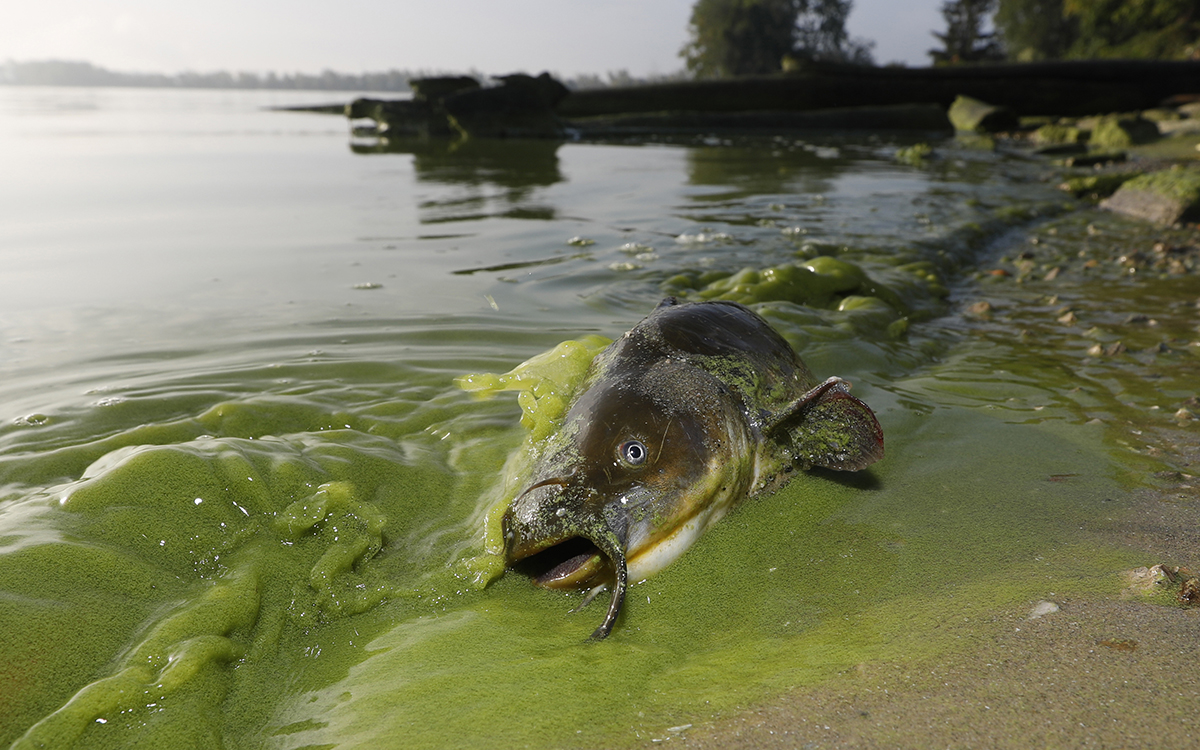
\includegraphics[width=0.6\textwidth]{figures/Algbloom.jpg}
    \caption{Water gevuld door algen in North Toledo, OHIO (US) | PHOTO BY ANDY MORRISON/THE BLADE VIA AP PHOTO}
    \label{fig:bloom}
\end{figure}

	\section{Theorie}
In dit onderzoek staat het creëren van een model van een ecosysteem centraal. De nadruk in dit model licht op hoe fytoplankton of 'Pythoplankton' concentratie verandert in een ecosysteem. In het bijzonder de jaarlijkse algen bloei en wat de effecten zijn van de mens hier op.\\

In dit ecosysteem wordt de biomassa van een populatie gemodelleerd door middel van de concentratie stikstof in de desbetreffende populatie. De redenen hiervoor zijn omdat  organisme vaste concentraties Stikstof nodig hebben om in leven te blijven. De hoeveelheid stikstof is in een gesloten ecosysteem behouden. Bovendien de stikstofkringloop overzichtelijk waardoor deze goed te modelleren is.\\

In de theorie wordt een versimpeld model uitgebreid tot een model met een variabele ruimtelijke dimensie in de diepe Ocean. Hierna wordt de fotosynthese snelheid onderzocht bovendien wordt er een stabiliteit analyse gedaan.
%Model

%misschien een beschrijving waar we naar toe gaan.
\subsection{Model}
De basis van dit model is een systeem met vier variabele grootheden. De diepte van de geheel gemixte laag $M(t)$, De concentratie Nutriënten $N(t)$, De concentratie Plankton $P(t)$ en de concentratie Herbivoren $H(t)$. Het gemoduleerde systeem is een afgebakend oppervlak in de diepe Ocean en alles wat zich onder dit oppervlak afspeelt. In dit model is er aangenomen dat de gehele plankton populatie zijn voedingstoffen verkrijgt uit fotosynthese. Verder is er aangenomen dat de zee een eindige gemixte laag heeft en dat alle organisme allen binnen deze geheel gemixte laag kunnen overleven.

\subsubsection{Lotka-Volterravergelijking}
Om het gehele model te kunnen beschrijven wordt eerst een versimpeling beschreven. Deze versimpeling bevat enkel De Plankton en de Herbivoren. De verandering van dit model wordt beschreven door de Lotka-Volterravergelijking te zien in figure \ref{eq reducedmodeldiff}.
\begin{equation}
    \begin{split}
        \frac{dP}{dt} &= \alpha(t) P-\frac{c(P-P_0)H}{K+P-P_0} \\[1ex] 
        \frac{dH}{dt} &= f\frac{c(P-P_0)H}{K+P-P_0}-gH\\[1ex] 
     \label{eq reducedmodeldiff}
    \end{split}
\end{equation}
Deze differentiaal vergelijkingen beschrijven hoe de populaties in de tijd veranderen. In de differentiaal vergelijkingen is de fotosynthesesenheid $\alpha(t)$ te zien samen met de overdracht van de Plankton naar de herbivoren door middel van 'eten' $\frac{c(P-P_0)}{K+P-P0}$. Ook is te zien dat de Herbivoren het systeem verlaten doordat deze op worden gegeten door carnivoren of sterven $-g$. 

\subsubsection{Evans \& Parslow (1985)}
In het verslag van Evans \& Parslow uit 1985 \cite{Algen1985} wordt de Lotka-Volterravergelijking van \ref{eq reducedmodeldiff} uitgebreid met de geheel gemixde laag en de nutrienten concentratie. Dit leid tot de volgende differentiaal vergelijking.
\begin{equation}
    \begin{split}
        \frac{dM}{dt} &= \zeta(t) \\[1ex] 
        \frac{dN}{dt} &= -\left[ \frac{\alpha(t,M,P)N}{j+N}-r \right] P+\frac{m+\zeta^+(t)}{M}(N_0-N) \\[1ex] 
        \frac{dP}{dt} &= \left[\frac{\alpha(t,M,P)N}{j+N}-r\right]P-\frac{c(P-P_0)H}{K+P-P_0}-\frac{m+\zeta^+(t)}{M}(N_0-N) \\[1ex] 
        \frac{dH}{dt} &= f\frac{c(P-P_0)H}{K+P-P_0}-gH-\frac{\zeta(t)}{M}H \\[1ex] 
    \end{split}
     \label{eq modeldiff}
\end{equation}

In deze differentiaal vergelijking is $\zeta(t)$ de verandering van de geheel gemixte laag met $\zeta^+(t)= max(0,\zeta(t))$.
$\alpha(t,M,P)$ de fotosynthese snelheid. Alle overige constanten worden beschreven in tabel \ref{table:consts}.

%% IK weet niet hoe ik hem op de goede plek krijg. Hij moet er gewoon direct onder of misschien naar de appendix
\begin{table}[H]
\begin{center}
 \caption{\label{table:consts}De constanten uit vergelijkingen \ref{eq reducedmodeldiff} en \ref{eq modeldiff} worden weergegeven in deze tabel. De waardes komen uit Evans \cite{Algen1985}.}
     \begin{tabular}{|c c c c|} 
     \hline
     beschrijving & constante & waarde & eenheid \\ [0.5ex] 
     \hline\hline
     Uptake half saturation & j & 0.5 & $mM m^{-3}$  \\ 
     \hline
     Plant metabolic loss & r & 0.07 & $d^{-1}$  \\
     \hline
     Diffusion rate & m & 3 & $md^{-1}$  \\
     \hline
     Deep nutrients & $N_0$ & 10 & $mM m^{-3}$ \\
     \hline
      maximum grazing rate & c & 1 & $d^-1$  \\
     \hline
     Grazing threshold & $P_0$ & 0.1 & $mM m^-3$\\
     \hline
      Grazing half saturation & K & 1.0 & $mM m^-3$\\
     \hline
      Grazing efficiency & f & 0.5 & -\\
     \hline
     Loss to carnivores & g & 0.07 & $d^-1$ \\ 
     \hline
     Maximum photosyntetic rate & Q & 2 & $d^{-1}$ \\
     \hline
     Light attenuation by water & k & 0.10 & $m^{-1}$ \\
     \hline
    \end{tabular}

\end{center}
\end{table}

\subsubsection{geheel gemixte laag diepte}
In diepe oceanen is er altijd een levensvatbare gemixte laag en een niet levensvatbare laag. Hoe diep de gemixte laag komt is afhankelijk van seizoen en van locatie. De verandering van de gemixte laag diepte $\zeta(t)$ uit vergelijking \ref{eq modeldiff} is zo gekozen dat de gemixte laag diepte $M(t)$ figuur \ref{fig:mixedlayerdept} beschrijft.\\
In ondiepere zeeën zoals de Noordzee is er slechts enkel tijdens een warme zomer spraken van een gemixte laag diepte. Dit model werkt dus enkel voor diepere oceanen. Bovendien wordt er aangenomen dat all het doden organische materiaal zinkt onder deze gemixte laag. hierdoor is er aan genomen dat er onder de gemixte laag een nagenoeg vaste concentratie nutriënten bevind.

\begin{figure}[H]
    \centering
    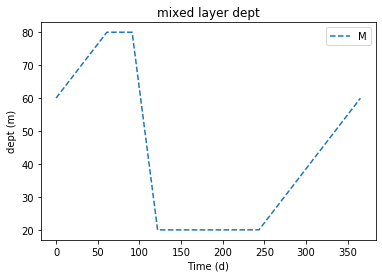
\includegraphics[width=0.33\textwidth]{figures/alpha/mixedlayerdept.png}
    \caption{De gemixte laag diepte tegen de tijd. De gemixte laag diepte is tijdens de zomer 20 meter en zakt na de winter naar de 80 meter diep. Deze grafiek is afkmostig uit \cite{Algen1985}.}
    \label{fig:mixedlayerdept}
\end{figure}

\subsubsection{fotosynthese snelheid}
De verandering in de Pythoplankton is onder ander afhankelijk van de fotosynthese snelheid, $\alpha$. Dit is de snelheid waarmee de pythoplankton nutriënten kan opnemen en is zoals de naam al aangeeft afhankelijk van fotosynthese. Er zijn meerdere componenten die dit beïnvloeden. In dit model is gefocust op de invloeden van de "Mixed layer depth", de seizoensgebondenheid en de concentratie pythoplankton en herbivoren. Er is gebruik gemaakt van de volgende formule \eqref{eq alpha}

\begin{equation}
    \alpha_{MHPt}(t,M,P)=\frac{2Q}{Mk}\left(g(\beta e^{kM},\tau)-g(\beta,\tau)-g(\beta e^{kM},0)+g(\beta,0) \right)\min(\frac{1}{\sqrt[3]{P+H}},1)\alpha_{seasonal}(t)
    \label{eq alpha}
\end{equation}
Waarin $g(y,t)=(y^2+t^2)^{\frac{1}{2}}-t\ln\left({\frac{t+(y^2+t^2)^{\frac{1}{2}}}{y}}\right)$ en $\beta=\frac{Q\tau}{\alpha J}$.
Hierin zijn de volgende waardes genomen, de relatieve daglengte,$\tau=0.5$, lage licht fotosynthese helling, $\alpha=4$ en licht level op het oppervlak in de middag, $J=2$.
De fotosynthese snelheid, $\alpha$ gebruikt in het verslag van Evans \& Parslow uit 1985 is genomen als de referentie voor de fotosynthese snelheid, $\alpha$.
De fotosynthese snelheid die uit functie \eqref{eq alpha} volgt is weergegeven in figuur \ref{alpha}. Ook de bijbehorende concentratie pythoplankton over de tijd is weergegeven.

\begin{figure}[H]
    \centering
    \subfloat[]{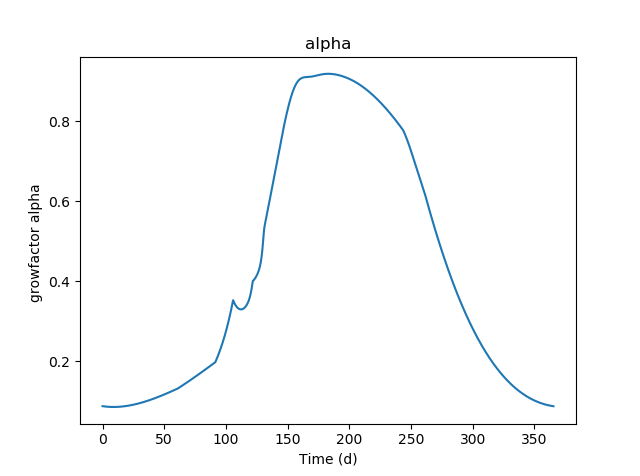
\includegraphics[width=0.5\textwidth]{figures/alpha/alphanormaal2.png}}
    \subfloat[]{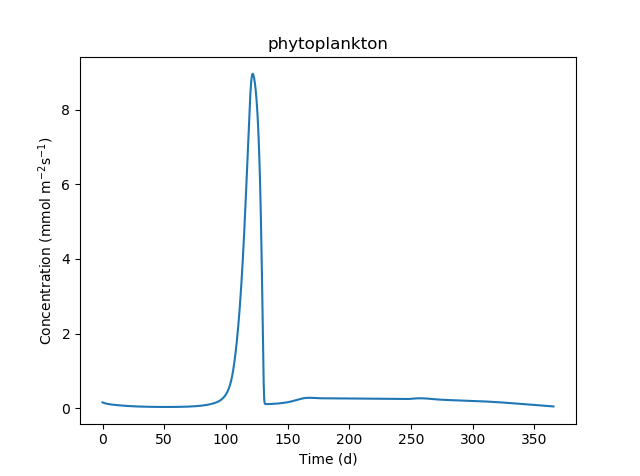
\includegraphics[width=0.5\textwidth]{figures/alpha/phytoplanktonnormaal2.png}}  
    
    \caption{(a) de fotosynthese snelheid over tijd die gebruikt is in dit model (b) De concentratie pythoplankton over tijd die uit deze fotosynthese snelheid volgt}
    \label{alpha}
\end{figure}

In het eerste deel van de functie (formule \eqref{eq alphaM}) is de afhankelijkheid van de "Mixed layer depth"\ te zien.
\begin{equation}
    \alpha_{M}(M)=\frac{2Q}{Mk}\left(g(\beta e^{kM},\tau)-g(\beta,\tau)-g(\beta e^{kM},0)+g(\beta,0) \right)
    \label{eq alphaM}
\end{equation}
Deze functie is verkregen uit de appendix van het verslag van Evans \& Parslow uit 1985 \cite{Algen1985}.
Er is ook duidelijk een verschil wanneer de fotosynthese snelheid afhankelijk en onafhankelijk is van de "mixed layer depth". 

\begin{figure}[H]

    \subfloat[]{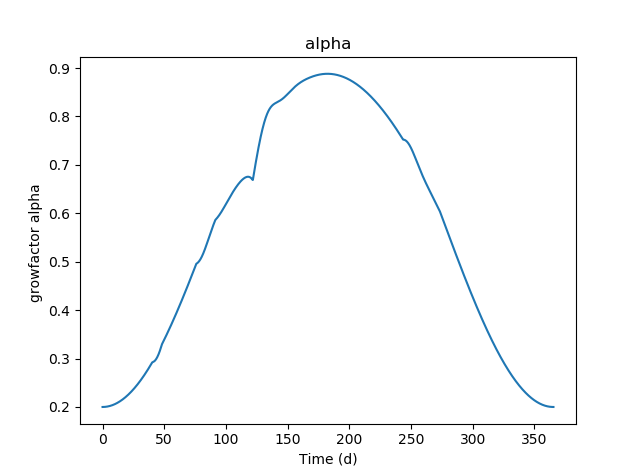
\includegraphics[width=0.5\textwidth]{figures/alpha/alphaMonafhankelijk2.png}}
    \subfloat[]{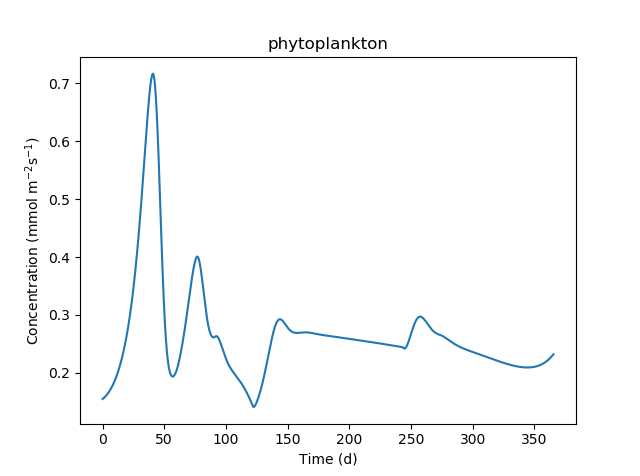
\includegraphics[width=0.5\textwidth]{figures/alpha/phytoplanktonMonafhankelijk2.png}}    

    \caption{(a) fotosynthese snelheid over tijd, onafhankelijk van de "Mixed layer depth" (b) De concentratie pythoplankton over tijd die uit deze fotosynthese snelheid volgt}
    \label{fig:alphamixedlayer}
\end{figure}
 
In figuur \ref{fig:alphamixedlayer}(a) is te zien dat voornamelijk de eerste periode van het jaar een duidelijk verschil is tussen de fotosynthese snelheid onafhankelijk en afhankelijk van de "Mixed layer depth". Dit zorgt ervoor dat er vrijwel geen bloei plaatsvindt, wat te zien is in \ref{fig:alphamixedlayer}(b). De pythoplankton concentratie bereikt hier hoogstens de waarde van $0.7 \frac{mmol}{m^2s}$, terwijl dit bij een normale bloei rond de $9 \frac{mmol}{m^2s}$ ligt. Een bloei is echter wel gewenst in dit model.
\\
\newline
De fotosynthese snelheid is ook afhankelijk van de hoeveelheid pythoplankton en herbivoren. Als de hoeveelheid pythoplankton en/of herbivoren namelijk erg groot wordt, gaat dit een deel van het licht blokkeren voor ander pythoplankton. Dit zorgt er dus voor dat deze geen zonlicht meer krijgen en de pythoplankton dus minder hard groeit (door minder fotosynthese). De fotosynthese snelheid is hier alleen voor afhankelijk als de pythoplankton en/of herbivoren concentratie heel hoog ligt, daarom is er voor een minimumfunctie gekozen. Als de concentratie pythoplankton en/of herbivoren erg hoog wordt zal de waarde van de functie $\alpha_P=min(\frac{1}{\sqrt[3]{P+H}},1)$ onder 1 komen en dus de fotosynthese snelheid dalen (wat er voor zorgt dat de groei van de pythoplankton daalt). Wanneer de concentratie pythoplankton en herbivoren laag is zal $\alpha_P=1$ gelden, waardoor de fotosynthese snelheid op dat moment niet afhankelijk is van de concentratie pythoplankton en herbivoren. 
Dit is te zien in figuur \ref{alphaPH}, wanneer de bloei van de pythoplankton plaatsvind (tussen de 100 en 150 dagen) is er een daling te zien in de fotosynthese snelheid en ook wanneer de concentratie herbivoren een piek heeft is een kleine daling te zien in de fotosynthese snelheid (tussen de 125 en 150 dagen).

\begin{figure}[H]
    \centering
    \subfloat[]{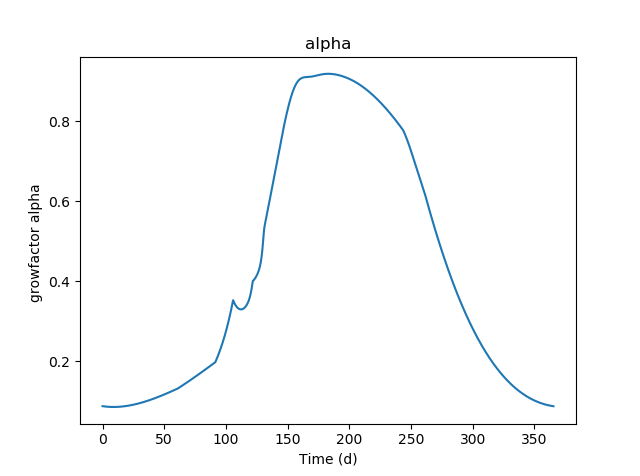
\includegraphics[width=0.5\textwidth]{figures/alpha/alphanormaal2.png}}
    \subfloat[]{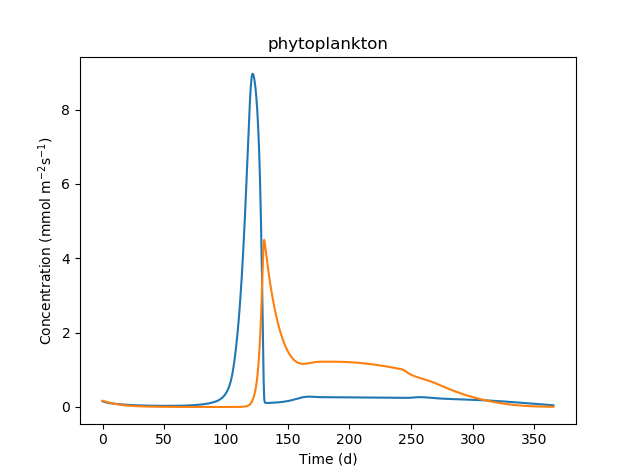
\includegraphics[width=0.5\textwidth]{figures/alpha/phytoplankton+herbnormaal2.png}}  
    
    \caption{(a) de fotosynthese snelheid over tijd die gebruikt is in dit model \\
    (b) Blauw: De concentratie pythoplankton over tijd die uit deze fotosynthese snelheid volgt\\
    Oranje: De concentratie Herbivoren over tijd die uit deze fotosynthese snelheid volgt.}
    \label{alphaPH}
\end{figure}

\\
De keuze voor $\frac{1}{\sqrt[3]{P+H}}$ in de afhankelijkheid is gemaakt aangezien dit de meest vergelijkbare fotosynthese snelheid gaf met de fotosynthese snelheid uit het verslag van Evans \& Parslow uit 1985. Hiervoor is een vergelijking te zien in de appendix.
\newline
\\
De laatste afhankelijkheid voor de door dit model gebruikte fotosynthese snelheid is de verandering in lichtintensiteit per seizoen. Zoals iedereen elk jaar merkt, is de lichtintensiteit in de zomer hoger dan in de winter. Dit heeft natuurlijk ook effect op de fotosynthese van pythoplankton. Hierdoor zal de fotosynthese snelheid in de winterperiode verzwakt zijn en in de zomerperiode niet. Hiervoor is er vermenigvuldigt met een cosinus functie $\alpha_{seasonal}=0.6-0.4\cos\left({\frac{2\pi}{365.25\tau}}\right)$. Deze heeft midzomer een top met $\alpha_{seasonal}=1$ en midwinter een dal met $\alpha_{seasonal}=0.6$. Deze waardes zijn weer gekozen omdat dit de meest vergelijkbare fotosynthese snelheid opleverde als bij het verslag van Evans \& Parslow. 
In figuur \ref{fig:alphaP} is te zien dat zonder de seizoensafhankelijke fotosynthese snelheid er weer vrijwel geen bloei plaatsvind, aangezien de concentratie pythoplankton hier $1.2 \frac{mmol}{m^2s}$ is in plaats van $9 \frac{mmol}{m^2s}$.


\begin{figure}[H]
    \centering
    \subfloat[]{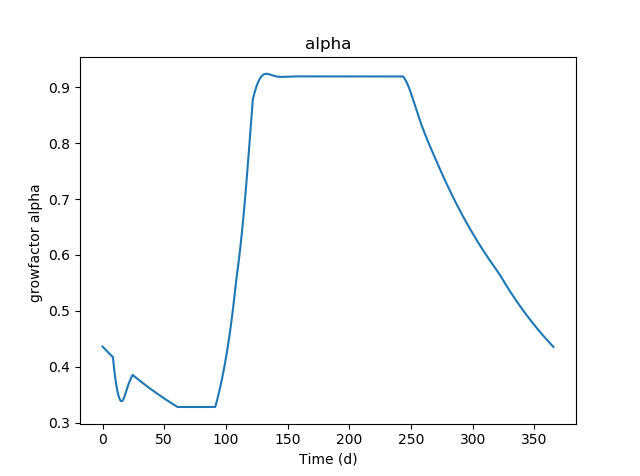
\includegraphics[width=0.5\textwidth]{figures/alpha/alphaSeizoenonafhankelijk2.png}}
    \subfloat[]{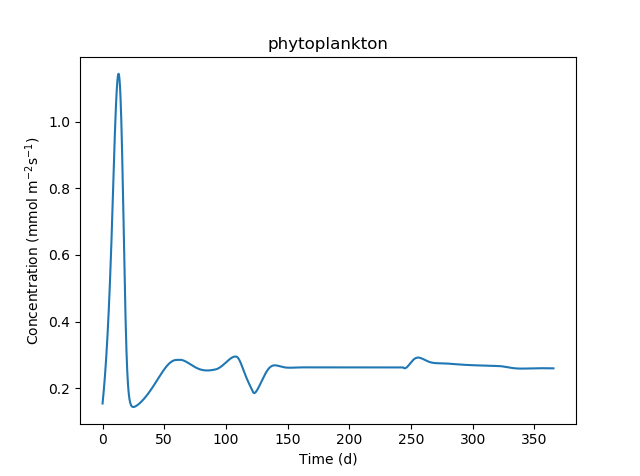
\includegraphics[width=0.5\textwidth]{figures/alpha/phytoplanktonseizoenonafhankelijk2.png}}

    \caption{(a) de fotosynthese snelheid onafhankelijk van het verschil in lichtintensiteit per seizoen (b) De concentratie pythoplankton over tijd die uit deze fotosynthese snelheid volgt}
    \label{fig:alphaP}
\end{figure}

In figuur \ref{fig:alphaEvans} is een vergelijking te zien tussen de fotosynthese snelheid die is gebruikt in dit model en de fotosynthese snelheid die is gebruikt in het verslag van Evans \& Parslow uit 1985. Hier is te zien dat in ze op veel punten overeenkomen. De vorm is bijna gelijk en er is bij beide een daling rond dezelfde tijdperiode (door de bloei van de pythoplankton). Er is echter wel een verschil in de pieken, deze verschillen namelijk lichtelijk van vorm en is bij de fotosynthese snelheid van dit model iets hoger. Dit kan meerdere oorzaken hebben. In het verslag van Evans \& Parslow uit 1985 is niet volledig beschreven waar ze hun fotosynthese snelheid op gebaseerd hebben. Dit kunnen dus ook andere factoren zijn dan de factoren die in dit model gekozen zijn. De fotosynthese snelheid is namelijk van vrij veel afhankelijk. 


\begin{figure}[H]
    \centering
    \subfloat[]{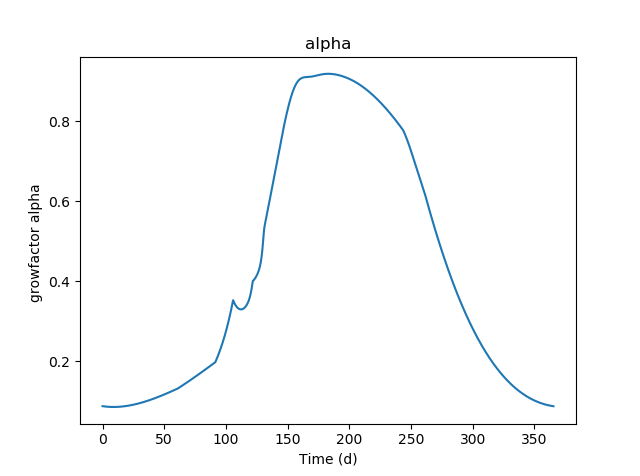
\includegraphics[width=0.5\textwidth]{figures/alpha/alphanormaal2.png}}
    \subfloat[]{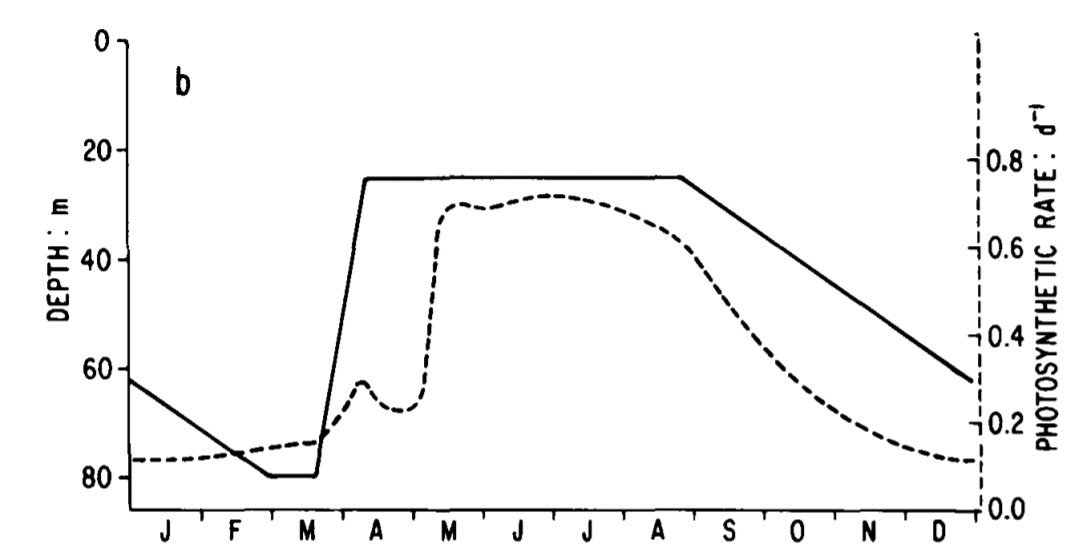
\includegraphics[width=0.5\textwidth, height=0.35\textwidth]{figures/alpha/evansparslowalpha.PNG}}

    \caption{(a) de fotosynthese snelheid over tijd die gebruikt in dit model (b) gestreepte lijn: de fotosynthese snelheid over tijd gebruikt in het verslag van Evans \& Parslow uit 1985 (doorgetrokken lijn: "mixed layer depth") \cite{Algen1985}
    }
    \label{fig:alphaEvans}
\end{figure}



\newpage
%Extra dimensie: nieuwe factoren
\subsection{Extra dimensie}
Laten we een één-dimensionaal kanaal beschouwen waarin we een concentratie noteren met $c(\vec{x},t)$. We nemen aan dat het kanaal zo dun is in de $y$ en $z$ richting dat we kunnen stellen dat $c(\vec{x},t)=c(x,t)$. Zie figuur \ref{fig:xchannel}

\begin{figure}[h]
	\centering
	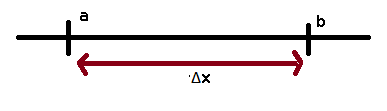
\includegraphics[]{DeltaX.png}
	\label{fig:xchannel}
	\caption{Stukje van het één dimensionale kanaal}
\end{figure}

Beschouw nu een interval $I_x$ tussen $x$ en $x+\Delta x$ met $\Delta x > 0$, dus $I_x = [x, x+\Delta x]$. De totale hoeveelheid stof verandert doordat er ofwel een netto flux is over de randen, ofwel er is bron. Naast dat er interne veranderingen zijn zoals beschreven in het model van Evans \& Parslow \cite{Algen1985}, introduceert de extra dimensie twee nieuwe factoren die verandering van concentratie teweeg brengt, namelijk stroming en diffusie. In de volgende twee paragrafen wordt afgeleid hoe deze factoren de concentratie distributie be\"{i}nvloeden.

\subsubsection{Diffusie}
De totale hoeveelheid stof $M(x,t)$ in het interval $I$ wordt gegeven door de volgende vergelijking
\begin{equation}
	M(x,t) = \int_x^{x+\Delta x} c(\tilde{x})\dif \tilde{x} \approx c(x)\Delta x
\end{equation}
hier is aangenomen dat $\Delta x$ erg klein is en $c$ voldoende glad zodat $c(\tilde{x}) \approx c(x)$ voor $\tilde{x} \in I_x$. Vervolgens kijken we naar de diffusie. Ficks wet stelt dat de diffusie flux $J$ proportioneel is met de negatieve gradient van de concentratie met proportionaliteitsconstante $D$. Dit betekent
\begin{equation}
	\vec{J}(\vec{x},t) = -D\cdot  \nabla c(\vec{x},t) \overEquals{1D} -D\cdot \dd{x} c(x,t).
\end{equation}
De concentratie binnen het kanaal verandert dus doordat er een influx is aan de randen, deze is gegeven door
\begin{equation}
	\phi_{\text{D}}(t) = \oint_{\partial I} \vec{J}(\vec{x},t)\cdot \dif \vec{S} \oneD J(a,t)-J(b,t) = -D\bigg(\dd{c}{x}(a,t) - \dd{c}{x}(b,t)\bigg)
\end{equation}

Hieruit volgt dat 
\begin{equation}
     \frac{d}{dt}{M}(t) = \dd{}{t} \bigg(c(x) A \Delta x\bigg) = A\phi_{D}(t) = -AD\bigg(\dd{C}{x}(a,t) - \dd{c}{x}(b,t)\bigg)
\end{equation}
\begin{equation}
    \dd{C}{t} \approx  \frac{D\bigg(\dd{c}{x}(x+\Delta x,t) - \dd{C}{x}(x,t)\bigg)}{\Delta x}
\end{equation}
en als we nu de limiet van $\Delta x$ naar nul nemen vinden we 
\begin{equation}
    \dd{c}{t}(x,t) = \dd{}{x}D\dd{c}{x} \overEquals{*} D\ddn{c}{x}{2}
\end{equation}
waar we bij (*) hebben aangenomen dat het medium zeewater zo goed als homogeen is en $D$ als constante beschouwd kan worden.

\newpage
\subsubsection{Stroming}
Voor stroming kunnen we een zelfde soort aanpak gebruiken als bij diffusie. Echter, nu is de vergelijking voor de flux anders. We hebben
\begin{equation}\phi_{in} = \vec{\phi}''_{in}  \cdot \vec{A}(x)=  c(x)\vec{V}(x) \cdot \vec{A}(x)
\label{eq:currentFlux1}
\end{equation}
\begin{equation}\phi_{out} = \vec{\phi}''_{out}\cdot \vec{A}(x+\Delta x) = c(x+\Delta x)\vec{V}(x+\Delta x) \cdot \vec{A}(x+\Delta x)
\label{eq:currentFlux2}
\end{equation}
Waar de accenten de ruimtelijke dimensie aangeeft, dus één accent betekent per lengte-eenheid, twee accenten per oppervlakte-eenheid, enzovoorts. Omdat $\vec{V} \perp \vec{A} \quad \forall \tilde{x} \in [0,L]$ kunnen we vergelijkingen \ref{eq:currentFlux1} en \ref{eq:currentFlux2} reduceren naar simpele producten. De tijdsafgeleide van de totale hoeveelheid stof is dus
\begin{equation}
    \dd{M}{t}(x,t) \approx A\Delta x\frac{\partial c}{\partial t} =  \phi_{in} - \phi_{out} = c(x)V(x)A - c(x+\Delta x)V(x+\Delta x)A
\end{equation} 
\begin{equation} \frac{\partial c}{\partial t} =  \frac{c(x)V(x) - c(x+\Delta x)V(x+\Delta x)}{\Delta x}
\end{equation}
\begin{equation} \frac{\partial c}{\partial t} =  \frac{\partial c}{\partial x}(x)V(x) + c(x)\cancelto{0}{\frac{\partial V}{\partial x}(x)} = \frac{\partial c}{\partial x}(x)V(x)
\end{equation}

\textbf{TO BE CONTINUED - JB, ik wil dit bovenste ook nog verbeteren. Heb het gevoel dat het rigoreuzer kan door met willekeurige $a,b$ te werken}

%Randvoorwaarden
\subsection{Randvoorwaarden}
\subsubsection{Dirichelet}
\subsubsection{Neumann}
\subsubsection{Gemengde randvoorwaarden} %Ik kan Dirichelet aan één kant, en Neumann aan de andere kant proberen - Joost
\subsubsection{Periodieke}

\newpage
\subsection{Algemene en numerieke stabiliteit van het Gereduceerde Model}
Stabiliteit analyses van een numerieke methode zijn belangrijk aangezien een numerieke methode convergent als en slechts als die stabiel en consistent is, dit is Lax's equivalence theorem. Convergentie is gewenst omdat de numerieke benadering dan convergeert naar de oplossing van het systeem, in andere woorden wordt de oplossing dan goed benaderd. De gebruikte numeriek methode, Runge Kutta 4, is in het algemeen consistent. Het is dus belangrijk om de stabiliteit van de gebruikte methode te toetsen.\\
Zoals nog zal blijken is het gereduceerde model(\textbf{VERWIJZING}) al vrij ingewikkeld voor een "in-depth" stabiliteit analyse, er zal dus ook niet gekeken worden naar de uitbreiding naar het 4-d model en het 1-dimensionale ruimtelijke model. Bij een stabiliteit analyse wordt gekeken naar de stabiliteit dichtbij de evenwichts-oplossing. Als er gekeken wordt naar (\textbf{VERWIJZING Reducedmodel}) wordt snel duidelijk dat er nooit een evenwicht zal ontstaan omdat $\alpha(t)$ periodiek is in de tijd. In dit hoofdstuk gebruiken we de volgende $\alpha(t)$:
\begin{equation}
    \alpha(t)=0.4-0.3 \cos \bigg(\frac{2\pi t}{365}\bigg)
\end{equation}
Hier is $t$ geven in dagen zodat de cosinus een periode heeft van 365 dagen. Gelukkig varieert $\alpha(t)$ langzaam genoeg zodat $\alpha(t)$ als een constante genomen kan worden als gekeken wordt naar de evenwichts-oplossing. De evenwichts-oplossing hangt in het algemeen af van deze constante waarde van $\alpha$, op zijn plaats hangt deze waarde af van de tijd waarop de $\alpha$ constant wordt genomen; De waarde zit in het interval [0.1 , 0.7] en noemen we $A$. De nieuwe functie, welke op een gegeven moment constant is, noemen we $\alpha^*(t)$.\\
Met behulp van deze $\alpha^*(t)$ zal er zich een evenwicht instellen. De evenwichts-waarden voor $P$ en $H$ kunnen berekend worden door de rechterkant van (\textbf{VERWIJZING Reducedmodel}) gelijk te stellen aan nul. We vinden dan dat \begin{equation}
    P=\frac{f P_0+g k-g P_0}{c f-g} \textrm{     ,     } H= Af\frac{(cfP_0+g(k-P_0))}{g(cf-g)}
\end{equation}
(\textbf{CHECK haakjes en subscripts}) 
Voor de gebruikte waardes voor de constantes volgt dat $P = 0.1162791$ en $H = 0.8305648*A$. Van het systeem kunnen we rond deze eigenwaarden een richtingsveld maken met behulp van Maple. Voor twee waarden van $A$ is dit weergegeven in Figuur \ref{fig:phasePortrait}. We zien dat in deze gevallen de evenwichten er grafisch stabiel uitzien.

\begin{figure}[H]
  \centering
  \subfloat[ ]{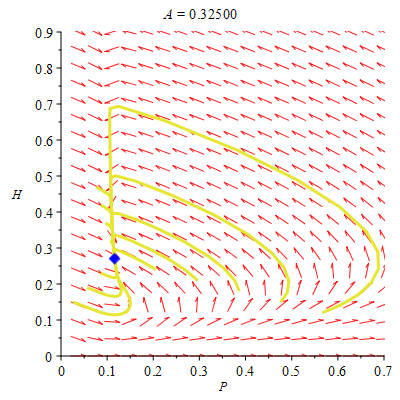
\includegraphics[width=0.5\textwidth]{figures/phase1.png}}
  \hfill
  \subfloat[ ]{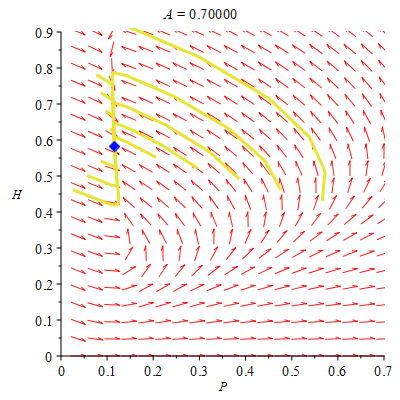
\includegraphics[width=0.5\textwidth]{figures/phase2.png}}
  \caption{Richtingsvelden voor het gereduceerde model voor waarden van de concentratie herbivoren $H$ en de concentratie phytoplankton $P$. Het evenwichtspunt is afhankelijk van A. Voor (a) en (b) is hier 0.325 en 0.7 gekozen respectievelijk. Gele lijnen geven oplossingen aan voor verschillende beginvoorwaarden. Deze afbeeldingen zijn gemaakt met Maple.}
  \label{fig:phasePortrait}
\end{figure}
Een deel van de gegeven voorbeeld oplossingen vertonen eerst ook een piek in de concentraties, waarna ze naar het evenwicht convergeren. Om te analyseren of de evenwichten analytisch stabiel zijn kijken we naar de linearisatie van het systeem. Deze wordt gekarakteriseerd door de Jacobiaan. Om te bepalen of een lineair systeem een stabiel evenwicht heeft wordt gekeken of de eigenwaarde van de karakteristieke matrix negatief zijn. Samengevat moet er gekeken worden naar het teken van de eigenwaarden van de Jacobiaan in het evenwichtspunt. De twee resulterende eigenwaarde zijn weergegeven in Figuur \ref{fig:eigen}.Uit het figuur is te zien. Dat alle eigenwaarden negatief zijn. Het evenwichtspunt is dus analytisch ook stabiel. \\
Er bestaat dus een fatsoenlijk kleine tijdstap zodat onze numerieke methode dus stabiel en dus convergent is. De voorwaarde voor de tijdstap kan berekend worden met de amplificatie-factor $A(\Delta t \lambda)$, als deze (strikt) kleiner is dan 1 zal de numerieke methode (absoluut) convergent zijn. De stabiliteitsvoorwaarde voor Runge-Kutta 4 is gegeven door
\begin{equation}
    A(\Delta t \lambda)=1+\Delta t \lambda+\frac{1}{2}(\Delta t \lambda)^2+\frac{1}{6}(\Delta t \lambda)^3+\frac{1}{24}(\Delta t \lambda)^4 \leq 1
\end{equation}

\begin{figure}[H]
  \centering
  \subfloat[ ]{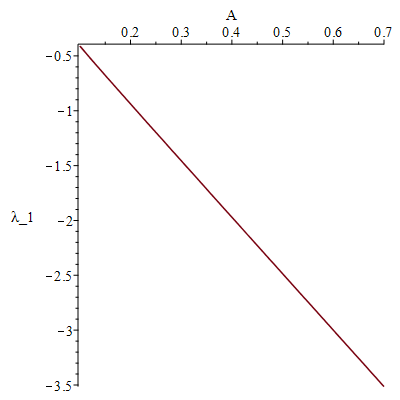
\includegraphics[width=0.5\textwidth]{figures/eigenwaarde1.png}}
  \hfill
  \subfloat[ ]{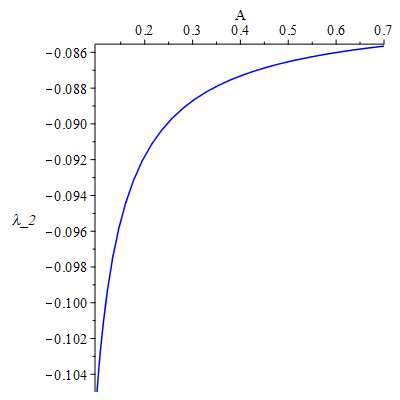
\includegraphics[width=0.5\textwidth]{figures/eigenwaarde2.png}}
  \caption{Eigenwaarden van de resulterende Jacobiaan. Deze zijn afhankelijk van $A$, de gekozen constante waarde van $\alpha(t)$. Beide waarde zijn negatief voor alle waarde van $A$.}
  \label{fig:eigen}
\end{figure}
Deze 4-de orde polynoom is enigszins lastig op te lossen, $\Delta t$ zal daarom grafisch worden afgeschat. De amplificatie-factor voor verschillende eigenwaarde is weergegeven in Figuur \ref{fig:AF}. Hier is de horizontale lijn met $y=1$ ook weergegeven. Uit de afbeelding is te zien dat voor $\Delta t \leq 0.78$ dagen de amplificatie factor onder de 1 ligt voor alle waarden van $A$. Hoe kleiner $A$ hoe lakser deze afschatting wordt. In de appendix wordt voor $A=0.7$ en $A=0.1$ de bijbehorende tijdstap afschatting getest met behulp van de numerieke methoden. Hier blijkt dat oplossingen, met een tijdstap die voldoet aan de afschatting, convergeren naar het berekende evenwicht. Oplossing, die niet een correcte tijdstap hebben, convergeren niet allemaal geheel correct. Sommigen zijn zelfs instabiel. De afschatting voor $\Delta t$ blijkt dus redelijk te kloppen.

\begin{figure}[H]
  \centering
  \makebox[\textwidth][c]{\subfloat[ ]{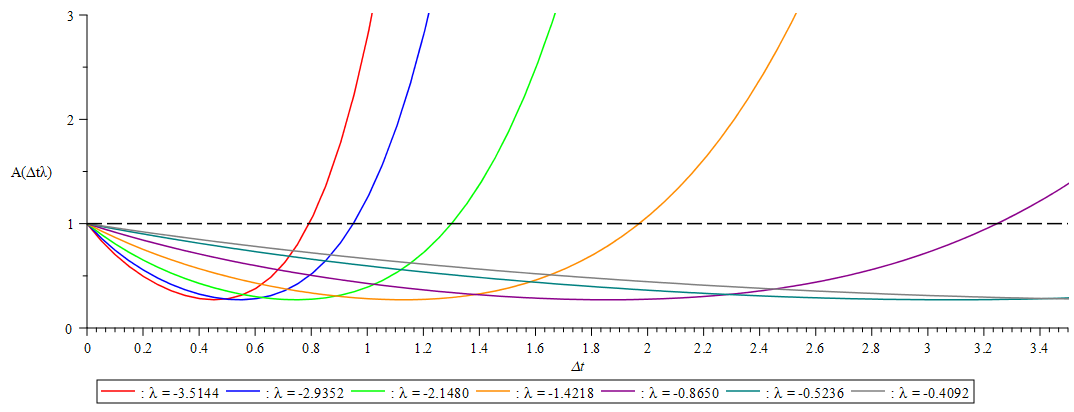
\includegraphics[width=1.2\textwidth]{figures/AmpFactor.png}}}
  \hfill
  \makebox[\textwidth][c]{\subfloat[ ]{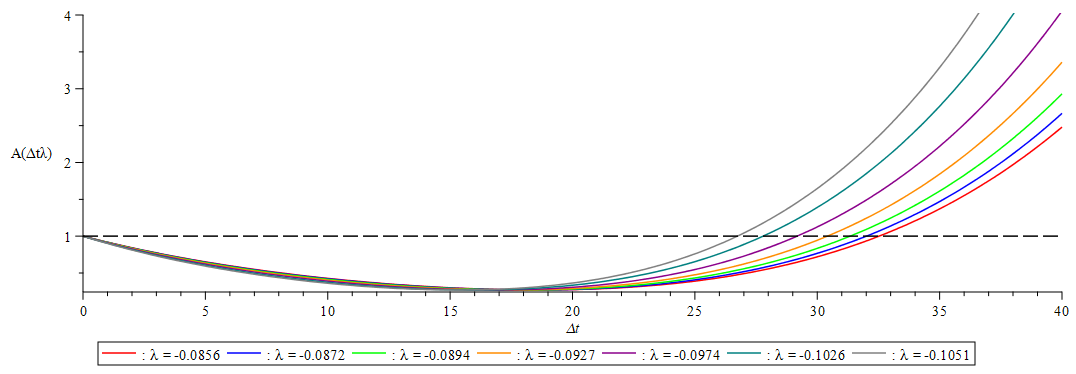
\includegraphics[width=1.2\textwidth]{figures/AmpFactor1.png}}}
  \caption{Amplificatie-factoren $A(\Delta t \lambda)$ weegegeven voor verschillende eigenwaarde $\lambda$. De kleinste en grootste eigenwaarde in beide afbeeldingen komen overeen met $A=0.1$ en $A=0.7$.}
  \label{fig:AF}
\end{figure}
	\section{Implementatie}
Om dit beginwaarden probleem op te lossen moet er een numerische integratie methode gebruikt worden. Neem een arbitraire continue functie $y(t)$ met als afgeleiden $f(t)$ dan wordt de waarden van $y(t)$ beschreven als volgt met $y(0)$ als begin waarden.
\begin{equation}
    \begin{split}
    \frac{d}{dt} y(t) &= f(t) \\
    y(t) &= y(0)+\int_{0}^t f(t)dt
    \end{split}
\end{equation}
In het algen model geldt $y(t)=\left[M(t), N(t), P(t), H(t) \right]^T$ \\
met respectievelijk $f(t)=\left[\frac{d}{dt}M(t), \frac{d}{dt}N(t), \frac{d}{dt}P(t), \frac{d}{dt}H(t) \right]^T$ uit vergelijking \ref{eq modeldiff}.

\subsection{Discretisatie afgeleiden}

\subsection{Numeriek integratie}
Een discretisatie is nodig om numeriek waardes te bepalen. De tijd wordt gediscretiseerd in tijdstappen met lengte $\Delta t$ hiermee is dus $t_n=n\Delta t$. De numerieke benadering van $y(t_n)$ wordt aangegeven met $W_n$. Om de numerische fout te minimaliseren wordt Runge-Kutta 4 gebruikt als numerieke integraties methode. Deze staat beschreven in vergelijking \ref{eq RK4}.
\begin{equation}
    \begin{split}
            W_{n+1} &= W_n+1/6(k_1+2k_2+2k_3+k_4)\\
            met\\
            k_1 &= \Delta t f\left(t_n,w_n\right)\\
            k_2 &= \Delta t f\left(t_n+\frac{\Delta t}{2},w_n+\frac{k_1}{2}\right)\\
            k_3 &= \Delta t f\left(t_n+\frac{\Delta t}{2},w_n+\frac{k_2}{2}\right)\\
            k_4 &= \Delta t f\left(t_n+\Delta t ,w_n+k_3\right)
            \label{eq RK4}
    \end{split}
\end{equation}

%% BORN:: NUMERIEK BOEK
%Runge-Kutta

\subsection{Python}
De numerieke integratie methode samen met de differentiaalvergelijkingen van \ref{eq modeldiff} en de stroming afhankelijkheid beschreven in [REVERENTIE] zijn geïmplementeerd in een geheel zelf geschreven python 3.6 code. Om alle waardes op te kunnen slaan is er gebruikt gemaakt van Numpy en voor de grafieken is Matplotlib gebruikt. Verdere informatie over de code en waar de code gevonden kan worden staat beschreven in de appendix.
	\section{Resultaten}
De
Hallo
[1-D model]
\begin{figure}[H]
    \centering
    \subfloat[]{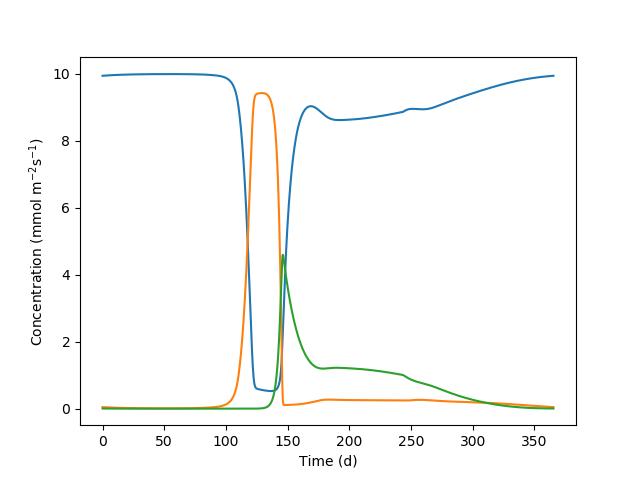
\includegraphics[width=0.5\textwidth]{figures/simple.png}}
    \subfloat[]{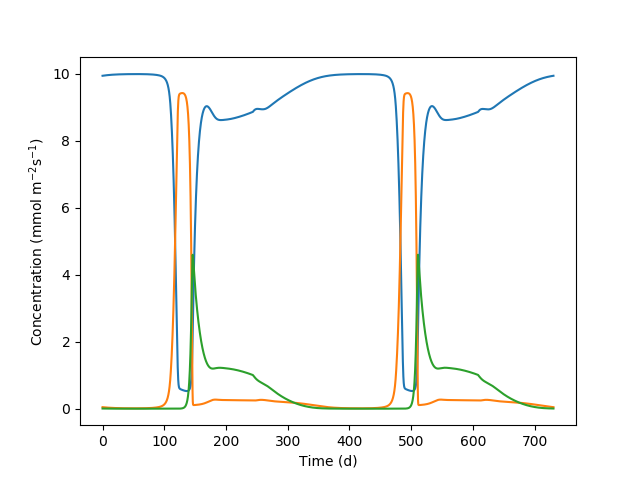
\includegraphics[width=0.5\textwidth, height=0.35\textwidth]{figures/simple_long.png}}

    \caption{Het één dimensionale model. De Nutrienten concentratie (blauw), plankton concentratie (orange) en de herbivoren concentratie (groen) weergegeven tegen de tijd. (a) tijd schaal van één jaar. (b) tijd schaal van twee jaar.
    }
    \label{fig:Res:Simple}
\end{figure}
In figuur \ref{fig:Res:Simple} is de jaarlijkse plankton bloei te zien die begint rond de 100ste dag na midwinter. Dit correspondeert aan eind maart of de begin van de lente. Na 30 dagen neemt de plankton concentratie weer af tot iets onder de gemiddelde waardes. Na de plankton piek is er te zien dat er een herbivoren concentratie piek is. De herbivoren concentratie blijft tot de 200ste dag relatief stabiel tot dat deze uiteindelijk ook afneemt.\\
\\
Om de ruimtelijke invloed te meten moet er gekozen worden voor een in ruimte varierende begin conditie. In dit onderzoek is er gekozen voor een gaussische begin conditie zoals zichtbaar in figuur \ref{fig:Res:IC}. Deze zou over een kunnen komen met een stikstof dumpend schip dat onlangs voorbij is gevaren.

\begin{figure}[H]
    \centering
    {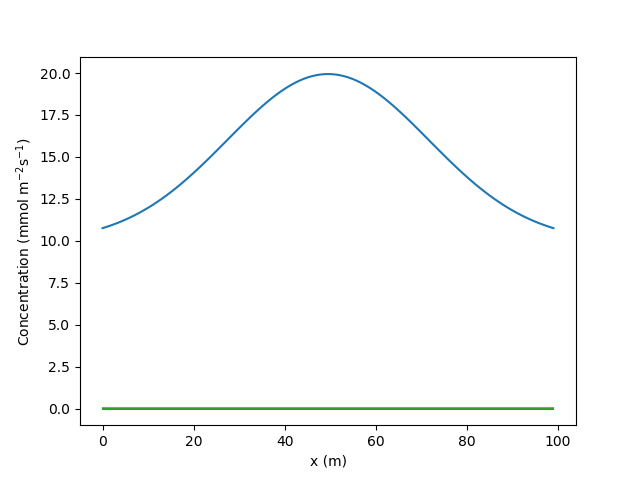
\includegraphics[width=0.5\textwidth]{figures/Inital_Condition.png}}
    \caption{ De begin conditie van het model met de Nutrienten concentratie (blauw), plankton concentratie (orange) en de herbivoren concentratie (groen). Hierin is te zien dat de stikstof concentratie een gausische curve beschrijft in de ruimte. Ook is te zien dat de begin waardes van de herbivoren en plankton concentratie plaats onafhankelijk zijn.
    }
    \label{fig:Res:IC}
\end{figure}

Om de effecten van de stroming en diffusie apart te kunnen analyseren zijn in figuur \ref{fig:Res:Color0} alle andere effecten uitgezet. 
\begin{figure}[H]
    \centering
    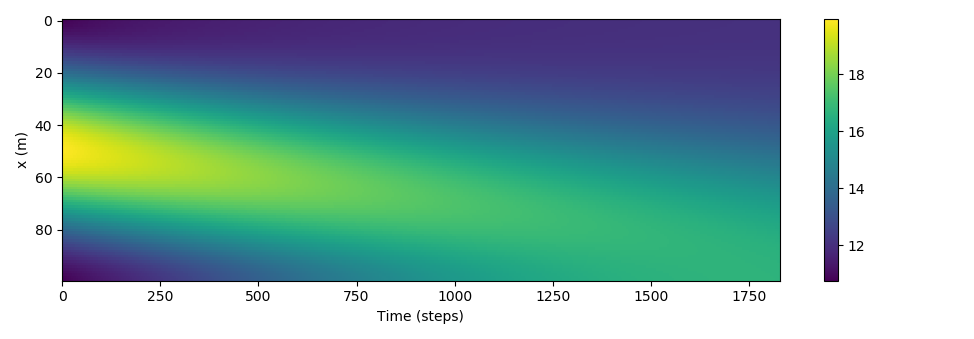
\includegraphics[width=0.8\textwidth]{figures/color_plot_0Flow.png}
   \hfill
    \caption{De invloed van enkel de stroming en diffusie op de begin conditie. Hierin is ruimte tegen de tijd weergegeven met de hierin de concentratie als kleur. Welke waarde met welke concentratie correspondeert is te zien in de bij staande legenda.}
    \label{fig:Res:Color0}
\end{figure}

In figuur \ref{fig:Res:Color0} is zichtbaar dat de gausisch beginwaarde van figuur \ref{fig:Res:IC} in breedte toeneemt terwijl de piek in hoogte afneemt en naar beneden verschuift door middel van de stroming.

\begin{figure}[H]
   \centering
   \subfloat[]{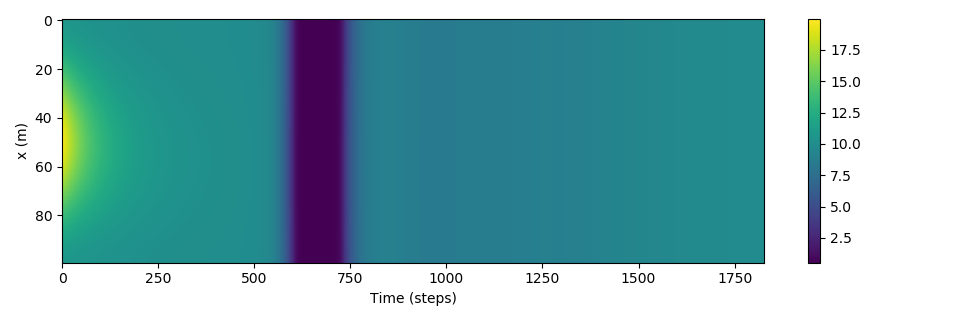
\includegraphics[width=0.5\textwidth]{figures/color_plot_1N.png}}
   \hfill
   \subfloat[]{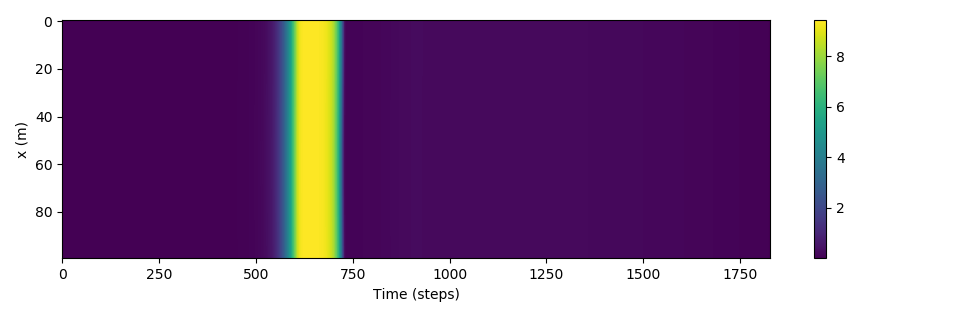
\includegraphics[width=0.5\textwidth]{figures/color_plot_1P.png}}
   \hfill   
   \subfloat[]{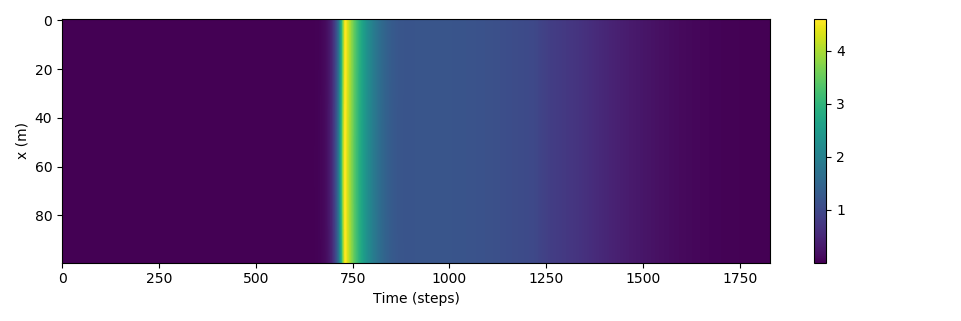
\includegraphics[width=0.5\textwidth]{figures/color_plot_1H.png}}
   \hfill
    \caption{}
    \label{fig:Res:Color1}
\end{figure}

\begin{figure}[H]
    \centering
   \subfloat[]{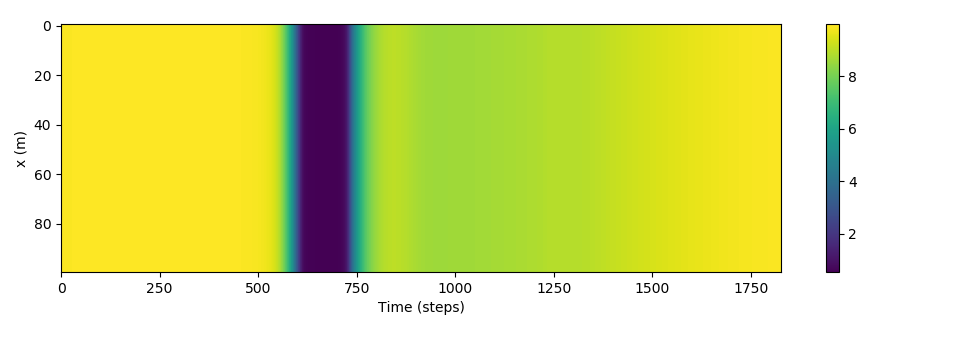
\includegraphics[width=0.5\textwidth]{figures/color_plot_1N2.png}}
   \hfill
   \subfloat[]{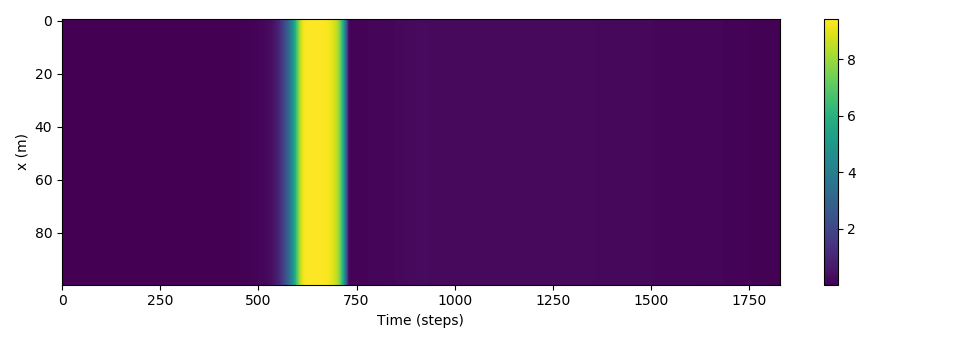
\includegraphics[width=0.5\textwidth]{figures/color_plot_1P2.png}}
   \hfill
   \subfloat[]{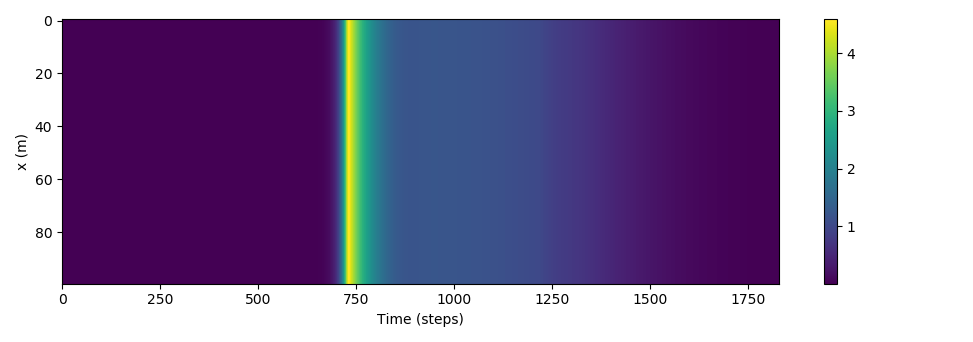
\includegraphics[width=0.5\textwidth]{figures/color_plot_1H2.png}}
   \hfill
   \caption{Caption}
   \label{fig:Res:Color2}
\end{figure}

\begin{figure}[H]
\centering
   \hfill
   \subfloat[]{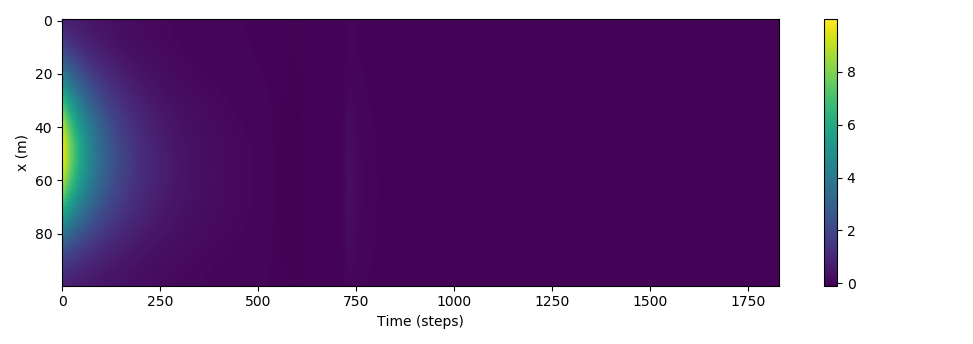
\includegraphics[width=\0.5\textwidth]{figures/color_plot_1N3.png}}
   \hfill
   \subfloat[]{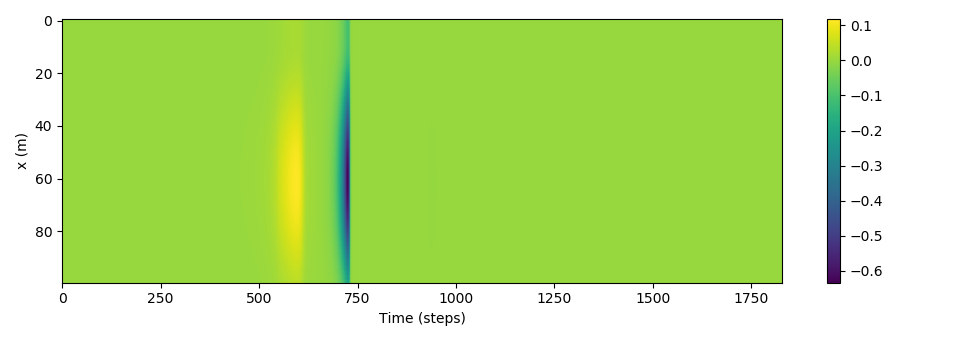
\includegraphics[width=0.5\textwidth]{figures/color_plot_1P3.png}}
   \hfill
   \subfloat[]{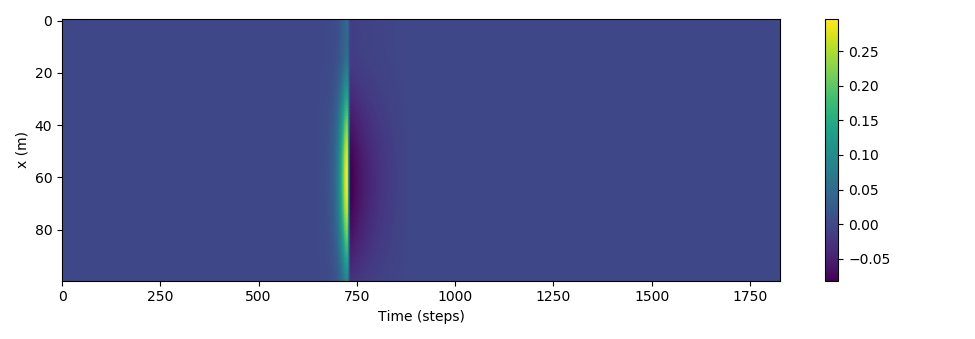
\includegraphics[width=0.5\textwidth]{figures/color_plot_1H3.png}}
   \hfill
   \caption{Caption}
    \label{fig:Res:Color3}
\end{figure}
	\section{Conclusie}

\subsection{Invloed beginvoorwaarden}

[ONS model voorspeld een bloei rond eind maart! aka de lente plankton bloei!

CONCULUSE: Ruimtelijke verranderingen zullen de Lente bloei niet of nauwelijks kunnen afremmen]
	\newpage
	
	%Bibliography

\printbibliography


 	\section*{Appendix}
\addcontentsline{toc}{section}{Appendix}

\subsection*{Code}
De python code die schreven is voor dit model is staat in een GitHup repository.\\
Deze is te vinden via de volgende link: 
https://github.com/bverhage/Algae\\
\\
Door de grootte van de code is er gekozen om de code te verdelen over verschillende documenten. Om de in dit verslag gebruikte resultaten te zien en de simulatie te runnen hoeft enkel het bestand met de naam 'Execution.py' gerund te worden. Een verdere beschrijving van de code staat op de GitHup webpagina.
\cite{artikel1}
\newpage
\subsection*{Testen stabiliteits-voorwaarde a.d.h. numerieke oplossing rond de evenwichts-oplossing}
In deze sectie zullen 2 tijdstap afschattingen grafisch gecheckt worden. Als we $A$ gelijk kiezen aan 0.7 zal de tijdstap kleiner 0.78 dagen.

\begin{figure}[H]
  \centering
  \makebox[\textwidth][c]{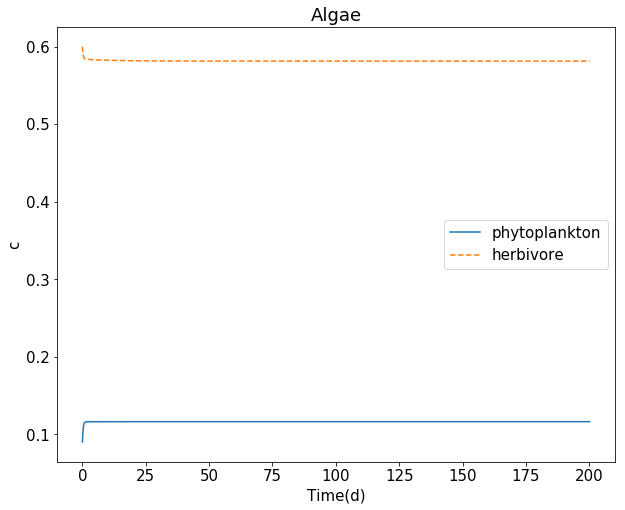
\includegraphics[width=0.4\textwidth]{figures/appendixstab/dt02.png}
  \hfill
  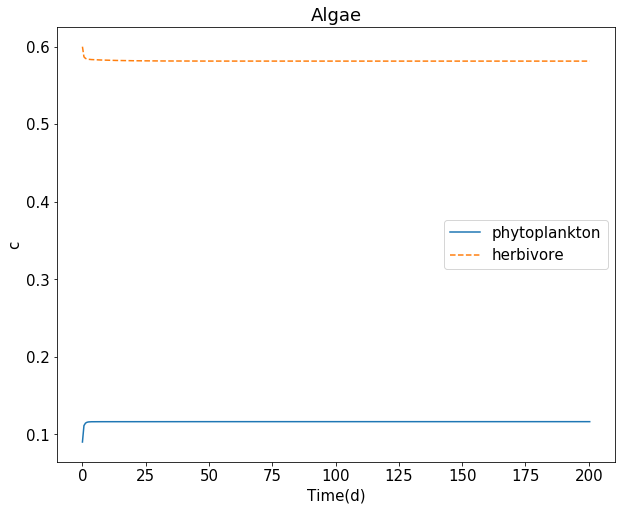
\includegraphics[width=0.4\textwidth]{figures/appendixstab/dt06.png}
  \hfill
  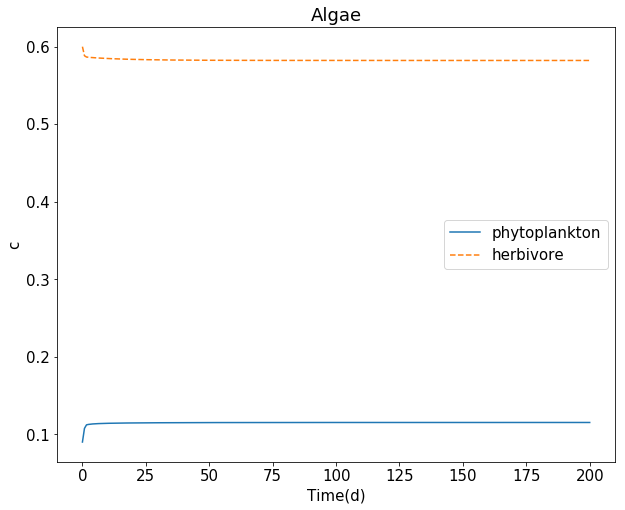
\includegraphics[width=0.4\textwidth]{figures/appendixstab/dt08.png}
    }
  \\
  (a):$\Delta t=0.2$ \hspace{0.27\textwidth} (b):$\Delta t=0.6$\hspace{0.27\textwidth}(c):$\Delta t=0.8$
  \makebox[\textwidth][c]{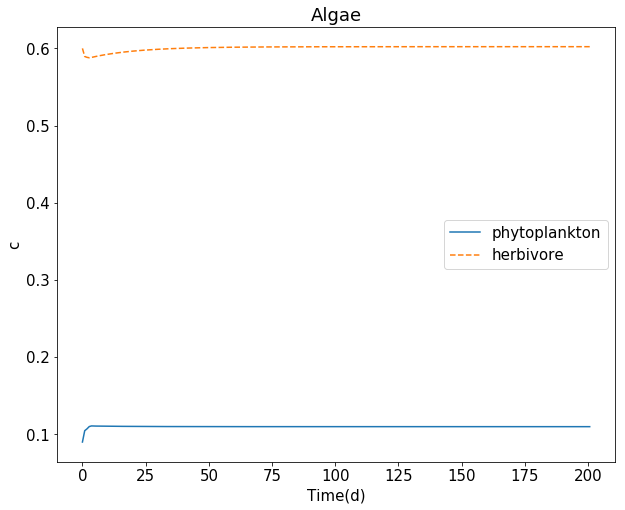
\includegraphics[width=0.4\textwidth]{figures/appendixstab/dt09.png}
  \hfill
  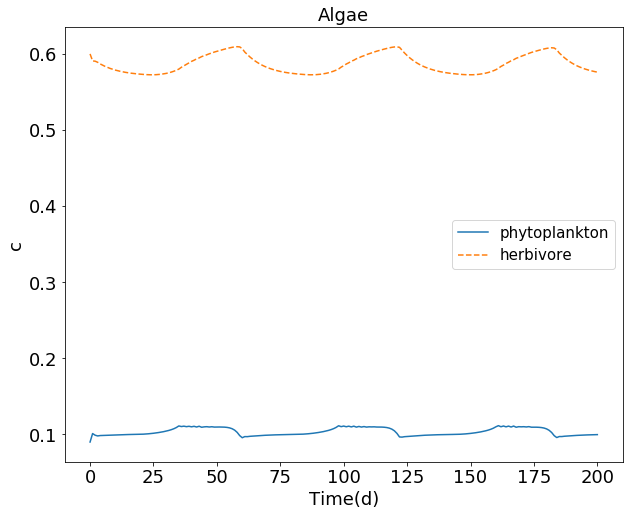
\includegraphics[width=0.4\textwidth]{figures/appendixstab/dt1.png}
  \hfill
  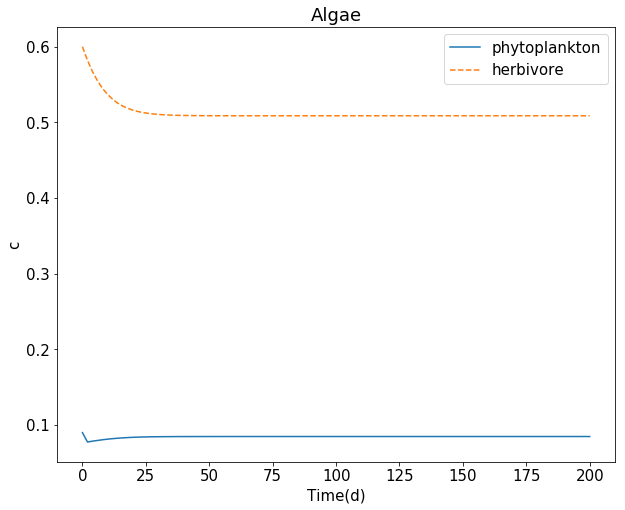
\includegraphics[width=0.4\textwidth]{figures/appendixstab/dt2.png}
    }
  \\
  (d):$\Delta t=0.9$ \hspace{0.28\textwidth} (e):$\Delta t=1$\hspace{0.28\textwidth}(f):$\Delta t=2$
  \centering
  \makebox[\textwidth][c]{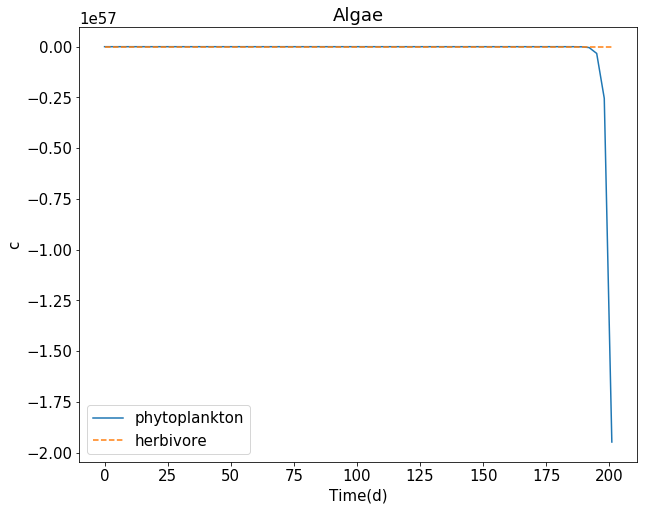
\includegraphics[width=0.42\textwidth]{figures/appendixstab/dt3.png}}
  (g):$\Delta t=3$
  \caption{Oplossingen van het gereduceerde model met een constante $\alpha(t)$, de constante waarde: $A=0.1$. Weergegeven zijn de concentratie $C$ van de phytoplankton en de herbivoren. De beginwaarde zijn dicht bij het evenwicht gekozen. De tijdstap is in dagen gegeven.}
  \label{fig:voorbeelden}
\end{figure} 
Oplossingen van het model voor deze tijdstap zijn weergegeven in Figuur \ref{fig:voorbeelden}, de beginwaarden liggen dichtbij het evenwicht. Voor (a),(b) en (c) convergeert de oplossing netjes naar het evenwicht. Bij (d) en (f) is het evenwicht een stukje verschoven van de $"$echte" waarden af. (e) en (g) convergeren duidelijk niet naar een evenwicht en zijn instabiel. Het blijkt dus dat de stabiliteits-voorwaarde redelijk klopt.\\
Voor $A=0.1$ zijn oplossingen weergegeven voor verschillende waarden van de tijdstap $\Delta t$ in Figuur \ref{fig:voorbeelden1}. Voor deze $A$ is het tijdstap criterium: $\Delta t \leq 0.67$. Hier convergeren de oplossingen die voldoen aan dit criterium, (a) en (b), naar het evenwicht. (c) convergeert al niet snel meer naar een evenwicht, het evenwicht is hier ook verschoven. Bij (d) zitten er al wat numerieke artefacten in. In (e) is de oplossing divergent en instabiel. Wederom blijkt de gevonden voorwaarde te kloppen.
\begin{figure}[H]
  \centering
  \makebox[\textwidth][c]{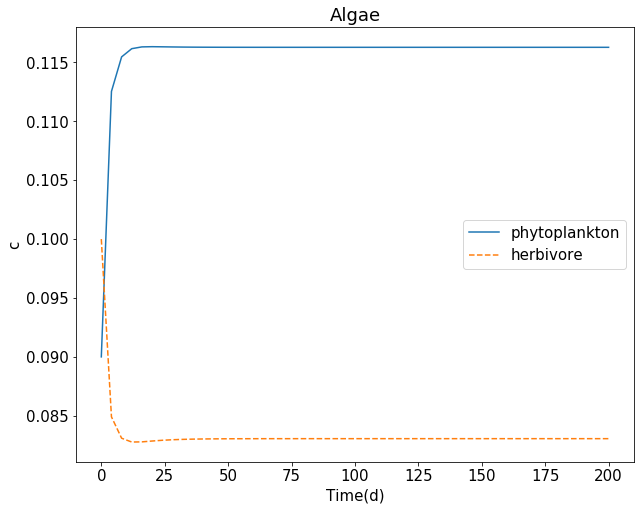
\includegraphics[width=0.4\textwidth]{figures/appendixstab/1dt4.png}
  \hfill
  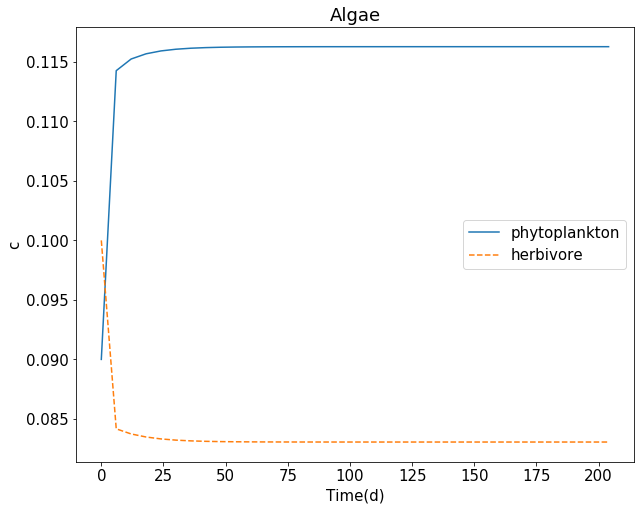
\includegraphics[width=0.4\textwidth]{figures/appendixstab/1dt6.png}
  \hfill
  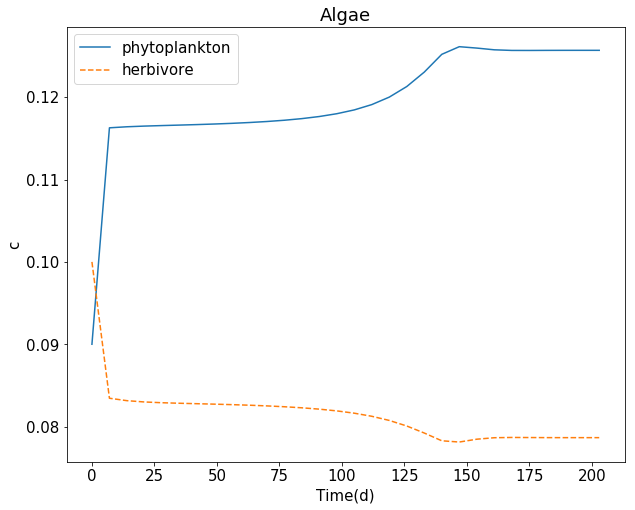
\includegraphics[width=0.4\textwidth]{figures/appendixstab/1dt7.png}
    }
  \\
  (a):$\Delta t=4$ \hspace{0.28\textwidth} (b):$\Delta t=6$\hspace{0.29\textwidth}(c):$\Delta t=7$
  \makebox[\textwidth][c]{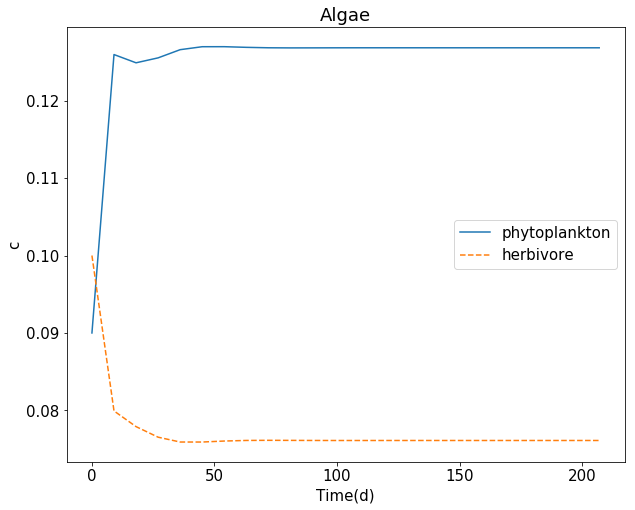
\includegraphics[width=0.4\textwidth]{figures/appendixstab/1dt9.png}
  \hfill
  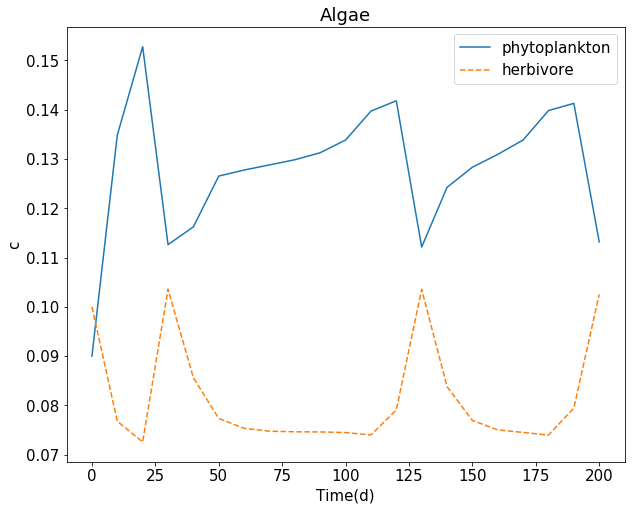
\includegraphics[width=0.4\textwidth]{figures/appendixstab/1dt10.png}
    }
  \\
  \hspace{0.11\textwidth}(d):$\Delta t=9$ \hspace{0.47\textwidth} (e):$\Delta t=10$\hspace{0.1\textwidth}
  \centering
  \caption{Oplossingen van het gereduceerde model met een constante $\alpha(t)$, de constante waarde: $A=0.1$. Weergegeven zijn de concentratie $C$ van de phytoplankton en de herbivoren. De beginwaarde zijn dicht bij het evenwicht gekozen. De tijdstap is in dagen gegeven. De verticale as verandert door de plaatjes heen. }
  \label{fig:voorbeelden1}
\end{figure} 

\newpage

\subsection*{afhankelijkheid fotosynthese van concentratie pythoplankton}

Er zijn verschillende verbanden getest in dit model voor de  afhankelijkheid van fotosynthese snelheid van concentratie pythoplankton. Er is uiteindelijk gekozen voor $\alpha_P=min(\frac{1}{\sqrt[3]{P}},1)$. Aangezien, zoals in figuur \ref{fig:alphavergelijking} te zien, deze een meest vergelijkbaar resultaat geeft met de fotosynthese snelheid uit het verslag van Evans \& Parslow. 

\begin{figure} [H]
    \centering
    \subfloat[]{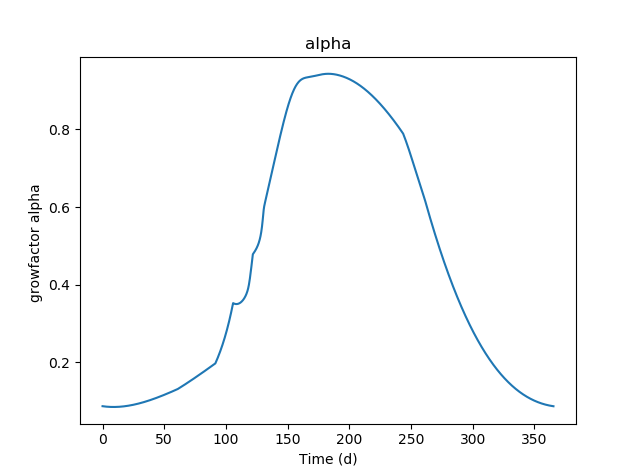
\includegraphics[width=0.35\textwidth]{figures/alpha/aplhaPH4.png}}
    \subfloat[]{\includegraphics[width=0.35\textwidth]{figures/alpha/alphaPH2.png}}
    \subfloat[]{\includegraphics[width=0.35\textwidth]{figures/alpha/AlphaPHe.png}}
    \\
    \subfloat[]{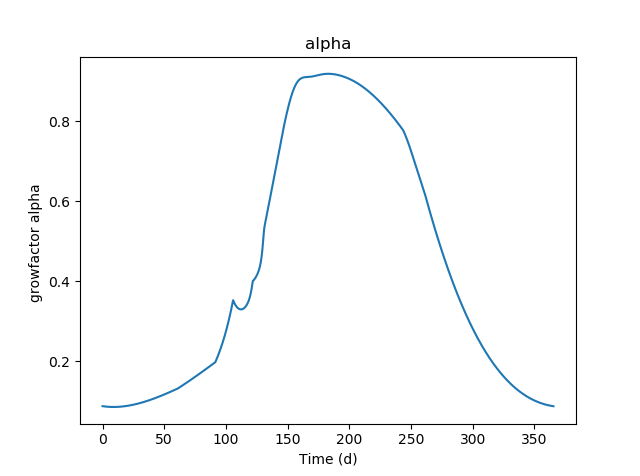
\includegraphics[width=0.4\textwidth]{figures/alpha/alphanormaal2.png}}
    \subfloat[]{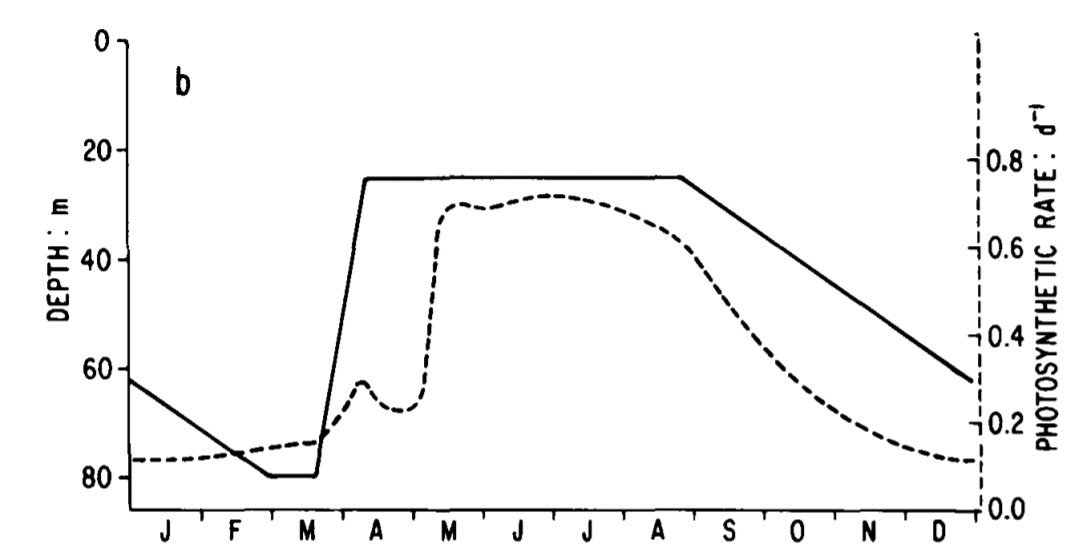
\includegraphics[width=0.5\textwidth]{figures/alpha/evansparslowalpha.PNG}}    
    \caption{  
    (a) De fotosynthese snelheid over tijd voor $\alpha_P=min(\frac{1}{\sqrt[4]{P+H}},1)$  
    (b) De fotosynthese snelheid over tijd voor $\alpha_P=min(\frac{1}{\sqrt[2]{P+H}},1)$  
    (c) De fotosynthese snelheid over tijd voor $\alpha_P=e^{-(P+H)}$ ($\leq 1$ , want $P \geq 0 $)  
    (d) De fotosynthese snelheid over tijd voor $\alpha_P=min(\frac{1}{\sqrt[3]{P+H}},1)$  
    (e) De fotosynthese snelheid over tijd uit het verslag van Evans \& Parslow uit 1985.}
    \label{fig:alphavergelijking}
\end{figure}


\end{document}
